\documentclass[11pt]{article}
\usepackage[margin=1in]{geometry}
\usepackage{tikz}
\usepackage{amsmath,amssymb}
\usepackage{xcolor}

\definecolor{tealA}{HTML}{9FE1CB}
\definecolor{tealB}{HTML}{5DCAA5}
\definecolor{tealC}{HTML}{1D9E75}
\definecolor{tealD}{HTML}{0F6E56}
\definecolor{tealE}{HTML}{085041}
\definecolor{coral}{HTML}{D85A30}

% zigzag worldline: #1 = number of round trips N, #2 = color. Velocity v=0.8, T=10 are fixed.
\newcommand{\zigzag}[2]{%
  \pgfmathsetmacro{\halfT}{5/#1}
  \pgfmathsetmacro{\amp}{0.8*\halfT}
  \pgfmathtruncatemacro{\nmax}{#1-1}
  \foreach \i in {0,...,\nmax} {
    \pgfmathsetmacro{\tzero}{\i*2*\halfT}
    \pgfmathsetmacro{\tmid}{\tzero+\halfT}
    \pgfmathsetmacro{\tend}{\tzero+2*\halfT}
    \draw[#2, line width=0.9pt] (0,\tzero) -- (\amp,\tmid) -- (0,\tend);
  }
}

\title{The reversed staircase:\\ proper time between two events can be arbitrarily small}
\author{}
\date{}

\begin{document}
\maketitle

\section{Setup}

Work in $1{+}1$-dimensional Minkowski space with coordinates $(x,t)$ and
$c=1$, so the interval is $ds^2 = dt^2 - dx^2$. For a timelike worldline
$x(t)$ with speed $|v(t)|=|dx/dt|<1$, the proper time elapsed is
$$\tau = \int \sqrt{1-v(t)^2}\;dt .$$

Fix two events at the same spatial location, separated by coordinate time
$T=10$:
$$A=(x{=}0,\,t{=}0), \qquad B=(x{=}0,\,t{=}10).$$
The simplest worldline joining them is the inertial one, $x\equiv 0$, with
proper time $\tau=T=10$.

\paragraph{This is the \emph{longest} timelike path.} For any curve
connecting $A$ to $B$, monotonic in $t$ from $0$ to $T$,
$$\tau=\int_0^T \sqrt{1-v(t)^2}\,dt \;\le\; \int_0^T dt = T,$$
with equality iff $v\equiv 0$. So the straight worldline maximizes proper
time -- the opposite of the Euclidean case, where the straight line
\emph{minimizes} length. This is the twin paradox in one line.

\section{A zigzag worldline}

Instead of sitting still, send the clock on $N$ identical round trips at
speed $v=0.8$: on trip $i$ it accelerates instantly, moves out to
$x=0.8\cdot T/(2N)$ and back, $N$ times, arriving back at $B$. Figure~\ref{fig:mink}
shows this for $N=1,2,4,8,16$, together with the inertial worldline (coral).

Each leg has duration $T/(2N)$ and speed $0.8$, so it contributes proper time
$\tfrac{T}{2N}\sqrt{1-0.8^2} = \tfrac{T}{2N}\cdot 0.6$. There are $2N$ legs, so
$$\tau_N = 2N\cdot\frac{T}{2N}\cdot 0.6 = 0.6\,T = 6,$$
independent of $N$ -- exactly as in the Euclidean staircase, refining the
zigzag does not change its total length. But here $6<10$: the zigzag is
\emph{shorter}, not longer, than the path it converges to. As $N\to\infty$
the trajectory's spatial excursion, $0.8\cdot T/(2N)\to 0$, so the worldline
converges uniformly to the straight line $x\equiv0$ -- yet its proper time
stays fixed at $6$, never approaching $10$.

\begin{figure}[h]
\centering
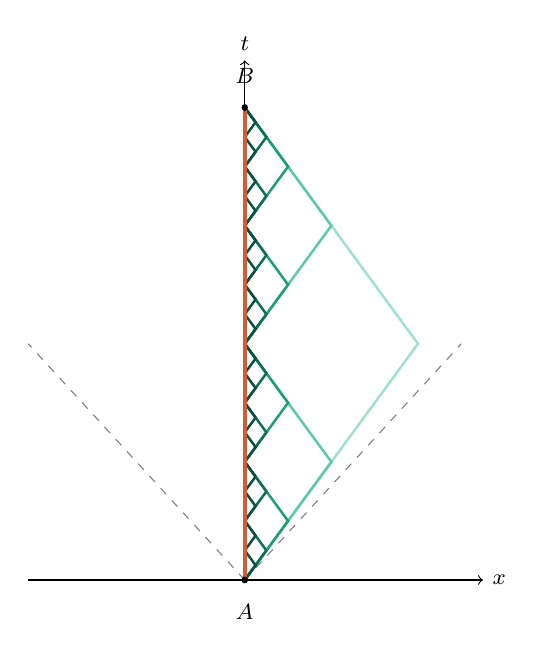
\begin{tikzpicture}[xscale=0.55,yscale=0.6]
  \draw[gray,dashed] (0,0) -- (5,5);
  \draw[gray,dashed] (0,0) -- (-5,5);
  \draw[->] (-5,0) -- (5.5,0) node[right,font=\footnotesize] {$x$};
  \draw[->] (0,0) -- (0,11) node[above,font=\footnotesize] {$t$};

  \zigzag{1}{tealA}
  \zigzag{2}{tealB}
  \zigzag{4}{tealC}
  \zigzag{8}{tealD}
  \zigzag{16}{tealE}

  \draw[coral, line width=1.6pt] (0,0) -- (0,10);

  \filldraw[black] (0,0) circle (0.06); \node[below,font=\footnotesize] at (0,-0.3) {$A$};
  \filldraw[black] (0,10) circle (0.06); \node[above,font=\footnotesize] at (0,10.3) {$B$};

\end{tikzpicture}

\vspace{1mm}
\begin{center}
\footnotesize
\tikz{\draw[tealA,line width=1.1pt](0,0)--(0.4,0);}~$N=1$ \quad
\tikz{\draw[tealB,line width=1.1pt](0,0)--(0.4,0);}~$N=2$ \quad
\tikz{\draw[tealC,line width=1.1pt](0,0)--(0.4,0);}~$N=4$ \quad
\tikz{\draw[tealD,line width=1.1pt](0,0)--(0.4,0);}~$N=8$ \quad
\tikz{\draw[tealE,line width=1.1pt](0,0)--(0.4,0);}~$N=16$ \\[1mm]
\tikz{\draw[coral,line width=1.8pt](0,0)--(0.4,0);}~inertial, $\tau=T=10$
\end{center}

\caption{Zigzag worldlines at $v=0.8$ with $N=1,2,4,8,16$ round trips between
the same two events $A$ and $B$, overlaid with the inertial worldline
(coral). Every zigzag, regardless of $N$, has proper time $\tau=6$; the
inertial line has $\tau=10$. Dashed gray lines mark the light cone at $A$.}
\label{fig:mink}
\end{figure}

\section{Proper time can be tuned to any value}

The velocity $0.8$ was just one choice. Repeating the computation for
general $v\in[0,1)$ gives, for any $N$,
$$\tau(v) = T\sqrt{1-v^2},$$
independent of $N$ and continuous and strictly decreasing in $v$, from
$\tau(0)=T$ down to $\tau(v)\to 0$ as $v\to 1$. Figure~\ref{fig:tau} plots
this. By the intermediate value theorem:

\begin{quote}
\textbf{Claim.} For every $\tau_0\in(0,T)$ there is a timelike worldline
from $A$ to $B$ with proper time exactly $\tau_0$: take any $v$ with
$\sqrt{1-v^2}=\tau_0/T$ and use the corresponding zigzag (any $N$ will do).
\end{quote}

So the proper time separating the \emph{same two events} is not fixed --
it can be made as close to $0$ as desired (though never reaching it for a
massive particle: $v=1$ is not attainable), while it can never exceed $T$,
which is reached only by the inertial worldline. In relativity, connecting
two timelike-separated events by an ever more agitated trajectory does not
add length, as it would in Euclidean geometry -- it erodes it, all the way
down to zero.

\begin{figure}[h]
\centering
\begin{tikzpicture}[xscale=6,yscale=5]
  \draw[->] (0,0) -- (1.08,0) node[right,font=\footnotesize] {$v$};
  \draw[->] (0,0) -- (0,1.08) node[above,font=\footnotesize] {$\tau/T$};
  \draw[thick,tealD,domain=0:1,samples=60,smooth,variable=\v] plot ({\v},{sqrt(1-\v*\v)});

  \draw[gray,dashed] (0.8,0) -- (0.8,0.6) -- (0,0.6);
  \filldraw[coral] (0.8,0.6) circle (0.015);
  \node[below,font=\footnotesize] at (0.8,-0.03) {$0.8$};
  \node[left,font=\footnotesize] at (-0.02,0.6) {$0.6$};

  \filldraw[black] (0,1) circle (0.015);
  \node[left,font=\footnotesize] at (-0.02,1) {$1$};
  \draw[black] (1,0) circle (0.015);
  \node[below,font=\footnotesize] at (1,-0.03) {$1$};
\end{tikzpicture}
\caption{$\tau/T=\sqrt{1-v^2}$: any target proper time in $(0,T)$ is reached
by some velocity $v\in(0,1)$. $v=0$ (filled dot) attains $\tau=T$; $v=1$
(open circle) is the unattained infimum $\tau=0$. The marked point is our
example, $v=0.8\Rightarrow\tau/T=0.6$.}
\label{fig:tau}
\end{figure}

\section{Why the sign is reversed}

For a short leg of coordinate duration $dt$ and speed $v$,
$$d\tau^2 = dt^2 - dx^2 = dt^2(1-v^2) \;\le\; dt^2,$$
whereas in Euclidean space the corresponding Pythagorean step reads
$$ds^2 = dx^2+dy^2 \;\ge\; dx^2.$$
Both are Pythagoras' theorem; the only difference is the minus sign coming
from the Lorentzian (indefinite) signature of the metric versus the
Euclidean (positive-definite) one. That single sign flip is why a detour
\emph{adds} length in Euclidean space -- as the staircase in the companion
note showed -- but \emph{subtracts} proper time here. It is also, precisely,
the mechanism behind the twin paradox: the twin who leaves and comes back
always ages less than the one who stays inertial, and the more violently
they move, the less they age -- with no lower bound above zero.

\section{Conclusion}

Two events with a fixed proper-time separation $T$ can be joined by
worldlines of any proper time in $(0,T)$: $T$ itself only by the straight,
inertial path, and values arbitrarily close to $0$ by fast enough zigzags,
even though every such zigzag converges, as a point set, to that same
straight worldline. This is the same phenomenon as the Euclidean staircase
-- length is not continuous under uniform convergence of curves -- but with
the inequality reversed: in Minkowski space the geodesic is the
\emph{longest} curve between two timelike-separated events, not the
shortest, and detours can erode proper time all the way to zero rather than
inflating length without bound.

\end{document}
